\chapter{Character Theory}
\thispagestyle{empty}

\begin{wrapfigure}[2]{r}{0.45\linewidth}
    \vspace{-15em}
    \centering
    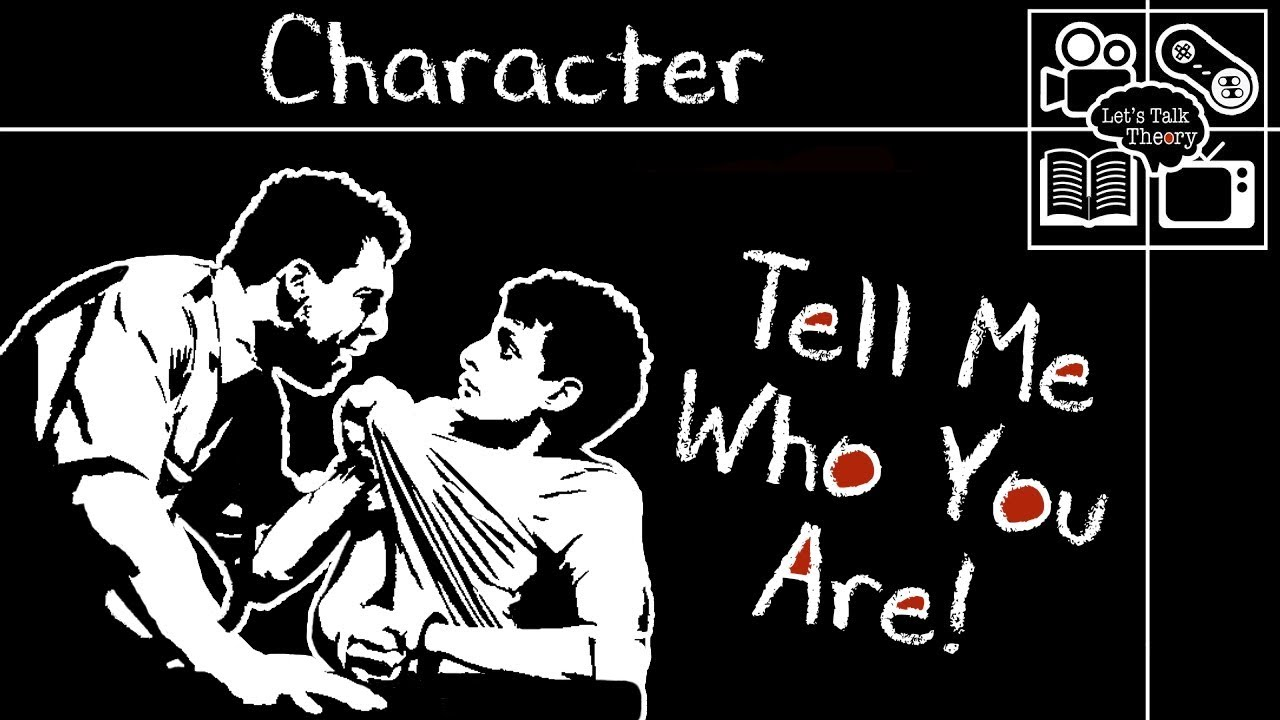
\includegraphics[width=0.8\linewidth]{./Chapters/2_Char/IMG_Char_Thy.jpg}
    \caption{\centering \small The thumbnail of a YouTube video titled ``What is Character Theory? $\vert$ Let's Talk Theory" by Dapper Mr. Tom. The video has nothing to do with mathematics.}
\end{wrapfigure}

In this chapter, we study an important type of functions from groups to fields known as characters. As we shall see, characters encode several useful properties of a group, and have been used extensively to prove several results about finite groups, (the representations of) which are the main object of study in this course. One of the reasons characters are useful to understand representation structures is that they are \textit{class functions}. That is, they encode information not about an individual element of a group but about its conjugacy class, making them good indicators of \textit{structural} and \textit{behavioural} properties. In particular, the character of a representation is independent of the choice of basis of the associated vector space.

Throughout this chapter, we denote by $G$ an arbitrary finite group.

\section{Preliminaries}

\subsection{Important Definitions and Properties}

\begin{boxdefinition}[Character]
    Let $V$ be a $\C G$-module. The character $\chi_v$ is the function $\chi_V : G \to \C$ given by $\chi_v(g) = \Tr{\rho(g)}$, where $\rho$ is the representation associated to $V$.
\end{boxdefinition}

\begin{remark}
    Since the trace is independent of our choice of basis, the definition makes sense.
\end{remark}

\begin{definition}[Irreducibility]
    We say a character $\chi_V$ is irreducible if the associated representation $\Vp$ is irreducible over $\C$.
\end{definition}
\begin{definition}[Degree]
    We define the degree of a character to be that of its associated representation.
\end{definition}
\begin{definition}[Trivial Character]
    We define the trivial character to be that associated with the trivial representation.
\end{definition}

\begin{proposition}[Behaviour of Characters]
    Let $V$, $W$ be $\C G$-modules, and let $g \in G$ be arbitrary. Then,
    \begin{enumerate}[label = \normalfont \arabic*., noitemsep]
        \item $\chi_{V \+ W} = \chi_V + \chi_W$
        \item $V \cong W \implies \chi_V = \chi_W$
        \item $\pdim{V} = \chi_V(1)$
        \item $\chi_v(g)$ is a sum of $d$th roots of unity, where $d = \ord{g}$.
        \item $\abs{\chi_V(g)} \leq \pdim{V}$
        \item $\chi_V\!\parenth{g\inv} = \overline{\xi_V(g)}$
    \end{enumerate}
\end{proposition}
\begin{proof}
    We do not give complete proofs here, just sketches.
    \begin{enumerate}
        \item This follows from the fact that the trace of a direct sum is the sum of the traces.
        \item This follows from the invariance of the trace under change of basis.
    \end{enumerate}
    \verb|sorry|
\end{proof}

\subsection{Character Tables}

A character table is exactly what it sounds like: a table consisting of the elements of a group, their images in a representation, and their associated characters. In this subsection, we investigate character tables by going through specific examples.

\begin{example}[The Dihedral Group of Order $8$]
    Let $G = D_8$, the dihedral group of order $8$. Consider the presentation
    \begin{align*}
        G = \cycl{a, b \mid a^4 = b^2 = 1, b\inv a b = a\inv}
    \end{align*}
    Let $\rho : G \to \GL{2, \C}$ be a representation of $G$ over $\C$ given by
    \begin{align*}
        \rho(a) = \begin{bmatrix}
            0 & 1 \\ -1 & 0
        \end{bmatrix}
        \quad\quad \text{ and } \quad\quad
        \rho(b) = \begin{bmatrix}
            1 & 0 \\ 0 & -1
        \end{bmatrix}
    \end{align*}
    We then have the following character table for $\rho$:
    \begin{table}[H]
        \centering
        \begin{tabular}{|c|cccccccc|}
            \hline
            $g$ & $1$ & $a$ & $a^2$ & $a^3$ & $b$ & $ab$ & $a^2 b$ & $a^3 b$ \\
            $\rho(g)$ &
            $\begin{bmatrix} 1 & 0 \\ 0 & 1 \end{bmatrix}$
            &
            $\begin{bmatrix} 0 & 1 \\ -1 & 0 \end{bmatrix}$
            &
            $\begin{bmatrix} -1 & 0 \\ 0 & -1 \end{bmatrix}$
            &
            $\begin{bmatrix} 0 & -1 \\ 1 & 0 \end{bmatrix}$
            &
            $\begin{bmatrix} 1 & 0 \\ 0 & -1 \end{bmatrix}$
            &
            $\begin{bmatrix} 0 & -1 \\ -1 & 0 \end{bmatrix}$
            &
            $\begin{bmatrix} -1 & 0 \\ 0 & 1 \end{bmatrix}$
            &
            $\begin{bmatrix} 0 & 1 \\ 1 & 0 \end{bmatrix}$
            \\
            $\chi_V(g)$ & $2$ & $0$ & $-2$ & $0$ & $0$ & $0$ & $0$ & $0$ \\
            \hline
        \end{tabular}
    \end{table}
\end{example}

\begin{example}[The Cyclic Group of Order $3$]
    Let $G = C_3 = \cycl{a}$ be the cyclic group of order $3$. Let $\rho_1, \rho_2, \rho_3$ be irreducible representations of $G$, with corresponding (irreducible) characters $\chi_1, \chi_2, \chi_3$.
\end{example}

\section{The Theory of Orthogonal Characters}

\subsection{On Central Functions}

\begin{boxdefinition}[Central Function]
    We say $f : G \to \C$ is central if $\fx = \fof{g\inv x g}$ for all $x,g \in G$.
\end{boxdefinition}

\begin{boxexample}[Examples of Central Functions]
    \hfill
    \begin{enumerate}
        \item The character of a $\C G$-module
        \item The order function $x \mapsto \ord{x} : G \to \N \subset \C$
    \end{enumerate}
\end{boxexample}

\begin{boxnotation}
    We define
    \begin{enumerate}
        \item $\Fof{G, \C} := \set{f : G \to \C}$
        \item $\Fcof{G, \C} := \set{f \in \Fof{G, \C} : f \text{ is central}}$
        \item $\delta_g(x)$ to be the indicator function (for $g, x \in G$).
    \end{enumerate}
\end{boxnotation}

\begin{remark}
    It turns out that $\Fof{G, \C}$ has the natural structure of being a $\C$-vector space of dimension $\abs{G}$, with basis $\set{\delta_g : g \in G}$.
\end{remark}

\begin{definition}
    Define $\cycl{\cdot, \cdot} : \FGC \times \FGC \to \C$ By
    \begin{align}
        \cycl{f_1, f_2} = \frac{1}{\abs{G}} \sum_{g \in G} f_1(g) \overline{f_2(g)}
    \end{align}
    One can show this to be an inner-product on $\FGC$.
\end{definition}

\subsection{The Orthogonality Theorem}

\begin{lemma}
    Let $\rho : G \to \GL{n, \C}$ and $\rho' : G \to \GL{m, \C}$ be irreducible representations of $G$ over $\C$. Fix $j, s \in \set{1, \ldots, m}$ and $r, i \in \set{1, \ldots, n}$.
    \begin{enumerate}[label = \normalfont \arabic*., noitemsep]
        \item If $\rho$ and $\rho'$ are \textit{not} equivalent, then
        \begin{align*}
            \frac{1}{\abs{G}} \sum_{g \in G} {\rho(g)}_{ri} {\rho'\!\parenth{g\inv}}_{js} = 0
        \end{align*}

        \item If $\rho$ and $\rho'$ \textit{are} equivalent, then
        \begin{align*}
            \frac{1}{\abs{G}} \sum_{g \in G} {\rho(g)}_{ri} {\rho'\!\parenth{g\inv}}_{js} =
            \begin{cases}
                \frac{1}{n} & \text{if } i = j \text{ and } r = s \\
                0 & \text{otherwise}
            \end{cases}
        \end{align*}
    \end{enumerate}
    where we use the notation $T_{ij}$ to refer to the $ij$th entry of the matrix of $T$.
\end{lemma}
\begin{proof}
    Let $V = \C^n$ and $W = \C^m$ be the two simple $\C G$-modules corresponding to $\rho$ and $\rho'$ respectively. The idea is to define a linear map that will allow us to use Schur's Lemma.

    For some chosen bases of $V$ and $W$, let $\phi_{ij} : W \to V$ be the $\C$-linear map given by the $n \times m$ matrix with $ij$th entry $1$ and all other entries $0$. Define
    \begin{align*}  % TODO: Make hat look nice
        \hat{\phi_{ij}} := \frac{1}{\abs{G}} \sum_{g \in G} \rho(g) \circ \phi_{ij} \circ \rho'\!\parenth{g\inv}
    \end{align*}
    By Theorem \ref{SP:Thm:Schur_fin_G_over_C}, $\hat{\phi_{ij}}$ is a $\C G$-module homomorphism from $W$ to $V$.
    \begin{enumerate}
        \item If $W \not\cong V$, we have $\hat{\phi_{ij}} = 0$. In particular,
        \begin{align*}
            0 &= \parenth{
                \frac{1}{\abs{G}} \sum_{g \in G} \rho(g) \circ E_{ij} \circ \rho'\!\parenth{g\inv}
            }_{rs} \\
            &= \frac{1}{\abs{G}} \sum_{g \in G} \brac{\rho(g) \circ E_{ij} \circ \rho'\!\parenth{g\inv}}_{rs} \\
            &= \sum_{k=1}^{n} \sum_{l=1}^{m} \frac{1}{\abs{G}} \sum_{g \in G} \brac{\rho(g)}_{rk} \brac{E_{ij}}_{kl} \brac{\rho'\!\parenth{g\inv}}_{ls} \\
            &= \frac{1}{\abs{G}} \sum_{g \in G} \brac{\rho(g)}_{ri} \brac{\rho'\!\parenth{g\inv}}_{js}
        \end{align*}

        \item Similarly, if $W \cong V$, we can view $\phi_{ij}$ as being given by the $n \times n$ matrix $E_{ij}$. Now, by Theorem \ref{SP:Thm:Schur_fin_G_over_C}, we know that
        \begin{align*}
            \hat{\phi_{ij}} &= \frac{1}{n} \Tr{E_{ij}} \cdot \id_V \\
            &= \frac{1}{n} \delta_{ij} \cdot \id_V
        \end{align*}
        We can then show the desired result using a similar computation.
    \end{enumerate}
\end{proof}
\begin{remark}
    As per Dr. Rizzoli, on the exam, it's more important to know the idea of such a proof than the specifics of \textit{which index goes where}.
\end{remark}

\begin{boxtheorem}[Orthogonality Theorem] \label{Ch2:Thm:Orth_Char}
    Let $S, T$ be irreducible $\C G$-modules.
    \begin{enumerate}[label = \normalfont \arabic*., noitemsep]
        \item If $S \not\cong T$, then $\cycl{\chi_S, \chi_T} = 0$.
        \item If $S \cong T$, then $\cycl{\chi_S, \chi_T} = 1$
    \end{enumerate}
    In other words, irreducible characters form an orthogonal system.
\end{boxtheorem}
\begin{proof}
    Let $P : G \to \GL{n, \C}$ and $Q : G \to \GL{m, \C}$ be the representations corresponding to $S$ and $T$. We know that
    \begin{align*}
        \cycl{\chi_S, \chi_T} &=
        \frac{1}{\abs{G}} \sum_{G \in G} \chi_S(g) \chi_T\!\parenth{g\inv} \\
        &= \frac{1}{\abs{G}} \sum_{g \in G} \Tr{P(g)} \Tr(Q\!\parenth{g\inv}) \\
        &= \frac{1}{\abs{G}} \sum_{g \in G} \parenth{\sum_{i = 1}^{n} \brac{P(g)}_{ii}}\parenth{\sum_{j=1}^{n} \brac{Q\!\parenth{g\inv}}_{jj}} \\
        &= \sum_{i=1}^{n} \sum_{j=1}^{m} \frac{1}{\abs{G}} \sum_{g \in G} \brac{P(g)}_{ii} \brac{Q\!\parenth{g\inv}_{jj}}
    \end{align*}
    We can then use the previous lemma to evaluate these sums.
\end{proof}

We have the following important corollary.

\begin{corollary}
    Up to isomorphism, there are finitely many irreducible $\C G$-modules.
\end{corollary}

\subsection{Irreducible Characters}

\begin{boxnotation}[Irreducilbe Characters]
    Denote by $\Irr{G}$ the subset of $\Fcof{G, \C}$ consisting of irreducible characters of $G$.
\end{boxnotation}

The Orthogonality Theorem tells us the following facts about Irreducible Characters.

\begin{proposition}[On the Behaviour of Irreducible Characters] \label{Ch2:Prop:Bhv_Irred_Char}
    \hfill
    \begin{enumerate}[label = \normalfont \arabic*., noitemsep]
        \item $\Irr{G}$ is a linearly independent set. In particular, $\abs{\Irr{G}} \leq \abs{G}$.
        
        \item Let $V = V_1 \+ \cdots \+ V_r$ be a $\C G$ module, with $V_i$ simple for $1 \leq i \leq r$. For any simple $\C G$ module $S$, the number of $V_i$s isomorphic to $S$ is given by $\cycl{\chi_V, \chi_S}$.
        
        \item Let $V, V'$ be $\C G$-modules. Then, $V \cong V' \iff \chi_V = \chi_{V'}$.
        
        \item A \CGM\ $V$ is simple iff $\cycl{\chi_V, \chi_V} = 1$.
    \end{enumerate}
\end{proposition}
\begin{proof}
    \hfill
    \begin{enumerate}[label = \normalfont \arabic*.]
        \item The linear independence follows immediately from the fact that $\Irr{G}$ form an orthonormal system. The inequality follows from the fact that all central functions are class functions: they agree for all conjugate elements of $G$. This means that $\pdim{\Fcof{G, \C}}$ is simply the number of conjugacy classes of $G$. Since $\pdim{\Fcof{G, \C}}$ must be at least $\abs{\Irr{G}}$ and the number of conjugacy classes of $G$ must be at most $\abs{G}$, we have the desired result.
        
        \item We know that $\chi_V = \chi_{V_1} + \cdots + \chi_{V_r}$. So,
        \begin{align*}
            \cycl{\chi_V, \chi_S} &= \cycl{\chi_{V_1} + \cdots + \chi_{V_r}, V_S} \\
            &= \text{sorry}
        \end{align*}

        \item 
        \begin{description}
            \item[$\parenth{\implies}$] Already seen. % TODO: PUT REFERENCE!
            \item[$\parenth{\impliedby}$] % Let $\Irr{G} = \set{\chi_1, \ldots, \chi_r}$.
            The multiplicity\footnote{Ie, the number of times it appears in the direct sum decomposition of $V$ into simple $\C G$-modules} of a simple \CGM\ $S$ in $V$ is given by $\cycl{\chi_V, \chi_S} = \cycl{\chi_{V'}, \chi_S}$. Then, a simple \CGM\ must have the same multiplicity in both $V$ and $V'$. % TODO: REFINE!!
        \end{description}

        \item 
        \begin{description}
            \item[$\parenth{\implies}$] Already seen. % TODO: PUT REFERENCE!
            \item[$\parenth{\impliedby}$] Let $\Irr{G} = \set{\chi_1, \ldots, \chi_r}$, with corresponding simple \CGM s $\set{V_1, \ldots, V_r}$. Denoting by $a_i$ the multiplicity of each $V_i$ in $V$, we have that
            \begin{align*}
                V &= V_1^{\+ a_1} \+ \cdots \+ V_r^{\+ a_r}
            \end{align*}
            where we use the notation $V_i^{\+ a_i}$ to mean $\underbrace{V_i \+ \cdots \+ V_i}_{a_i \text{ times}}$.

            We then have
            \begin{align*}
                \chi_V &= \sum_{i=1}^{r} a_i \chi_i \\
                \implies \cycl{\chi_V, \chi_V} &= \sum_{i=1}^{r} a_i^2
            \end{align*}
            This means only one of the $a_i$s is nonzero, and equal to $1$. % WHAT????
        \end{description}
    \end{enumerate}
\end{proof}

We now have everything we need to prove the following important theorem.

\begin{theorem}
    $\Irr{G}$ is a basis for $\Fcof{G, \C}$.
\end{theorem}
\begin{proof}
    Let $W = \Span{\Irr{G}} \leq \Fcof{G, \C}$, with orthogonal complement $W^\perp$ with respect to the inner-product \verb|insert reference|. Since $V = W \+ W^\perp$, if we can show that $W^\perp = \set{0}$, we would have that $V = W$, proving the desired result.

    Fix $f \in W^\perp$, and consider the element $\hat{f} \in \C G$ given by  % CHANGE NOTATION!
    \begin{align*}
        \hat{f} &= \sum_{g \in G} \overline{f(g)} \cdot g
    \end{align*}

    First, we show that $\hat{f} \in \Zof{\C G}$---ie, that $\hat{f}$ commutes (multiplicatively) with all elements of $\C G$. To show this, it suffices to show that $h\inv \hat{f} h = \hat{f}$ for all $h \in G$. So, fix $h \in G$. Then,
    \begin{align*}
        h\inv \hat{f} h &=
        \sum_{g \in G} \overline{f(g)} \cdot h\inv g h \\
        &= \sum_{g \in G} \overline{\fof{h\inv g h}} \cdot h\inv g h \\ % Can take h\inv g h inside f because f is central. Mention somewhere.
        &= \hat{f}(g)
    \end{align*}
    where the last equality follows from a change of variables in the summation.

    Now, let $S$ be any simple \CGM. One can show that the map  % DOMAIN AND CODOMAIN????
    \begin{align*}
        \phi : S \to S : v \mapsto \hat{f} \cdot v
    \end{align*}
    is a \CGM\ homomorphism. % Include more details
    Then, by Theorem \ref{SP:Thm:Schur_fin_G_over_C}, we have that
    \begin{align*}
        \hat{f} &= \frac{1}{\pdim{S}} \Tr{\hat{f}\vert_S} \cdot \id
    \end{align*}
    We then have that
    \begin{align*}
        \Tr{\hat{f}\vert_S} &= \Tr{\sum_{g \in G} \overline{f(g)} \cdot g\vert_{S}} \\
        &= \sum_{g \in G} \overline{f(g)} \chi_S(g) \\
        &= \abs{G} \cycl{\underbrace{\chi_S}_{\in W}, \underbrace{f}_{\in W^\perp}} = 0
    \end{align*}
    proving that in fact, $\hat{f}\vert_S = 0$.
    
    \verb|sorry| % Use photo on phone to complete proof.
\end{proof}

\subsection{More Character Tables}

For the purposes of this subsection, let $C_1, \ldots, C_k$ be the conjugacy classes of $G$ with representatives $g_1, \ldots, g_k$ respectively. Recall that by the Orbit-Stabiliser Theorem,
\begin{align*}
    \abs{C_i} &= \frac{\abs{G}}{\abs{C_G(g_i)}}
\end{align*}
where $C_G(\cdot)$ refers to the centraliser\footnote{Recall that the centraliser of a group element is the set of all elements that commute with it.} of an element in $G$. Now, let $\Irr{G} = \set{\chi_1, \ldots, \chi_k}$.

\begin{boxdefinition}[Character Table]
    A character table is a $k \times k$ table whose columns are the conjugacy classes (or their representatives) and whose rows are the irreducible characters. In other words, it is a table whose $\parenth{i,j}$th entry is $\chi_i(g_j)$.
    % Maybe draw this...
\end{boxdefinition}

We now have the following important result that lets us check orthogonality as we go across the columns.

\begin{boxproposition}[First Orthogonality Relation]
    Given $1 \leq r, s \leq k$, we have
    \begin{align*}
        \frac{1}{\abs{G}} \sum_{j=1}^{k} \abs{C_j} \chi_r\!\parenth{g_j} \chi_s\!\parenth{g_j\inv} &= \delta_{rs}
    \end{align*}
\end{boxproposition}
\begin{proof}
    Observe that
    \begin{align*}
        \delta_{rs} &=
        \cycl{\chi_r, \chi_s} \\
        &= \frac{1}{\abs{G}} \sum_{g \in G} \chi_r(g) \chi_s\!\parenth{g\inv} \\
        &= \frac{1}{\abs{G}} \sum_{j=1}^{k} \parenth{\sum_{g \in C_i} \chi_r(g) \chi_s\!\parenth{g\inv}} \\
        &= \frac{1}{\abs{G}} \sum_{j=1}^{k} \abs{C_j} \chi_r\!\parenth{g_j} \chi_s\!\parenth{g_j\inv}
    \end{align*}
    where the last inequality follows from the fact that characters are central (ie, they are equal for all elements of a conjugacy class).
\end{proof}

We can use this to prove an important result about the regular representation.

\begin{theorem}
    Let $\chi_{\reg}$ denote the character of the regular representation of $G$ over $\C$. Then,
    \begin{align*}
        \chi_{\reg} &= \sum_{j=1}^{k} \chiof{j}{1} \chi_j
    \end{align*}
\end{theorem}
\begin{proof}
    \verb|sorry|  % From phone
\end{proof}

\begin{corollary}
    $\sum_{i=1}^{k} \parenth{\chiof{i}{1}}^2 = \abs{G}$.
\end{corollary}
\begin{proof}
    $\chiof{\reg}{1} = \sum_{i=1}^{k} \parenth{\chi_i(1)}^2 = \abs{G}$.
\end{proof}

We now have a similar result about going down the rows.

\begin{boxproposition}[Second Orthogonality Relation]
    Given $1 \leq r, s \leq k$, we have
    \begin{align*}
        \sum_{i=1}^{k} \chiof{i}{g_r} \chiof{i}{g_s\inv} =
        \begin{cases}
            0 &\text{ if } r \neq s \\
            \abs{C_G(g_r)} &\text{ if } r = s
        \end{cases}
    \end{align*}
\end{boxproposition}
\begin{proof}
    Let $A$ be the matrix $\parenth{A_{ij}}_{ij}$, where $A_{ij} := \chiof{i}{g_j}$. Similarly, let $B$ be the matrix $\parenth{B_{ij}}_{ij}$, where $B_{ij} := \frac{\abs{C_i}}{\abs{G}} \chiof{j}{g_i\inv}$. Then, writing $AB = \parenth{AB}_{pq}$, we have
    \begin{align*}
        \parenth{AB}_{pq} &=
        \sum_{l=1}^{k} A_{pl} B_{lq} \\
        &= \sum_{l=1}^{k} \chiof{p}{g_l} \frac{\abs{C_l}}{\abs{G}} \chiof{q}{g_l\inv} \\
        &= \cycl{\chi_p, \chi_q} = \delta_{pq}
    \end{align*}
    This proves that in fact, $AB = I$, the identity matrix. This, in particular, means that $BA = I$ as well. It turns out that setting $\delta_{pq} = \parenth{BA}_{pq}$ gives us the desired result. % TODO: COMPLETE!!!!!!!!!
\end{proof}

\begin{boxexample}[The Character Table of $S_3$]
    $S_3$ has precisely three conjugacy classes $C_1$, $C_2$ and $C_3$ with representatives $g_1 = 1$, $g_2 = \parenth{1 2}$ and $g_3 = \parenth{1 2 3}$. We then have the following character table for $S_3$:
    \begin{table}[H]
        \centering
        \begin{tabular}{c|ccc}
            & $1$ & $\parenth{12}$ & $\parenth{123}$ \\
            \hline
            $\chi_1$ & $1$ & $1$ & $1$ \\
            $\chi_2$ & $1$ & $-1$ & $1$ \\
            $\chi_3$ & $2$ & $0$ & $-1$
        \end{tabular}
    \end{table}
    Here, $\chi_1$ corresponds to the trivial representation (of degree $1$), $\chi_2$ to the sign representation (of degree $1$), and $\chi_3$ to the subrepresentation $W = \Span{e_1 - e_2, e_1 - e_3}$ (of degree $2$) of the permutation representation on $\C^3$. Note that all of these representations are irreducible, the first two because their degrees are $1$, and the third because we can show $\cycl{\chi_W, \chi_W}$ to be equal to $1$ (cf. the fourth point of Proposition \ref{Ch2:Prop:Bhv_Irred_Char}).
\end{boxexample}


\section{More Character Tables}

\subsection{The Orthogonality Relations}

For the purposes of this subsection, let $C_1, \ldots, C_k$ be the conjugacy classes of $G$ with representatives $g_1, \ldots, g_k$ respectively. Recall that by the Orbit-Stabiliser Theorem,
\begin{align*}
    \abs{C_i} &= \frac{\abs{G}}{\abs{C_G(g_i)}}
\end{align*}
where $C_G(\cdot)$ refers to the centraliser\footnote{Recall that the centraliser of a group element is the set of all elements that commute with it.} of an element in $G$. Now, let $\Irr{G} = \set{\chi_1, \ldots, \chi_k}$.

\begin{boxdefinition}[Character Table]
    A character table is a $k \times k$ table whose columns are the conjugacy classes (or their representatives) and whose rows are the irreducible characters. In other words, it is a table whose $\parenth{i,j}$th entry is $\chi_i(g_j)$.
    % Maybe draw this...
\end{boxdefinition}

We now have the following important result that lets us check orthogonality as we go across the columns.

\begin{boxproposition}[First Orthogonality Relation] \label{SP:1st_Orth_Rel}
    Given $1 \leq r, s \leq k$, we have
    \begin{align*}
        \frac{1}{\abs{G}} \sum_{j=1}^{k} \abs{C_j} \chi_r\!\parenth{g_j} \chi_s\!\parenth{g_j\inv} &= \delta_{rs}
    \end{align*}
\end{boxproposition}
\begin{proof}
    Observe that
    \begin{align*}
        \delta_{rs} &=
        \cycl{\chi_r, \chi_s} \\
        &= \frac{1}{\abs{G}} \sum_{g \in G} \chi_r(g) \chi_s\!\parenth{g\inv} \\
        &= \frac{1}{\abs{G}} \sum_{j=1}^{k} \parenth{\sum_{g \in C_i} \chi_r(g) \chi_s\!\parenth{g\inv}} \\
        &= \frac{1}{\abs{G}} \sum_{j=1}^{k} \abs{C_j} \chi_r\!\parenth{g_j} \chi_s\!\parenth{g_j\inv}
    \end{align*}
    where the last inequality follows from the fact that characters are central (ie, they are equal for all elements of a conjugacy class).
\end{proof}

We can use this to prove an important result about the regular representation.

\begin{theorem} \label{Ch2:Thm:Reg_Rep_Col_1}
    Let $\chi_{\reg}$ denote the character of the regular representation of $G$ over $\C$. Then,
    \begin{align*}
        \chi_{\reg} &= \sum_{j=1}^{k} \chiof{j}{1} \chi_j
    \end{align*}
\end{theorem}
\begin{proof}
    \verb|sorry|  % From phone
\end{proof}

\begin{corollary} \label{Ch2:Cor:Reg_Rep_Col_1_Grp_Size}
    $\sum_{i=1}^{k} \parenth{\chiof{i}{1}}^2 = \abs{G}$.
\end{corollary}
\begin{proof}
    $\chiof{\reg}{1} = \sum_{i=1}^{k} \parenth{\chi_i(1)}^2 = \abs{G}$.
\end{proof}

We now have a similar result about going down the rows.

\begin{boxproposition}[Second Orthogonality Relation]
    Given $1 \leq r, s \leq k$, we have
    \begin{align*}
        \sum_{i=1}^{k} \chiof{i}{g_r} \chiof{i}{g_s\inv} =
        \begin{cases}
            0 &\text{ if } r \neq s \\
            \abs{C_G(g_r)} &\text{ if } r = s
        \end{cases}
    \end{align*}
\end{boxproposition}
\begin{proof}
    Let $A$ be the matrix $\parenth{A_{ij}}_{ij}$, where $A_{ij} := \chiof{i}{g_j}$. Similarly, let $B$ be the matrix $\parenth{B_{ij}}_{ij}$, where $B_{ij} := \frac{\abs{C_i}}{\abs{G}} \chiof{j}{g_i\inv}$. Then, writing $AB = \parenth{AB}_{pq}$, we have
    \begin{align*}
        \parenth{AB}_{pq} &=
        \sum_{l=1}^{k} A_{pl} B_{lq} \\
        &= \sum_{l=1}^{k} \chiof{p}{g_l} \frac{\abs{C_l}}{\abs{G}} \chiof{q}{g_l\inv} \\
        &= \cycl{\chi_p, \chi_q} = \delta_{pq}
    \end{align*}
    This proves that in fact, $AB = I$, the identity matrix. This, in particular, means that $BA = I$ as well. It turns out that setting $\delta_{pq} = \parenth{BA}_{pq}$ gives us the desired result. % TODO: COMPLETE!!!!!!!!!
\end{proof}

\subsection{Character Tables of Symmetric Groups}

\begin{example}[$S_3$]
    $S_3$ has precisely three conjugacy classes $C_1$, $C_2$ and $C_3$ with representatives $g_1 = 1$, $g_2 = \parenth{1 2}$ and $g_3 = \parenth{1 2 3}$. We then have the following character table for $S_3$:
    \begin{table}[H]
        \centering
        \begin{tabular}{c|ccc}
            & $1$ & $\parenth{12}$ & $\parenth{123}$ \\
            \hline
            $\chi_1$ & $1$ & $1$ & $1$ \\
            $\chi_2$ & $1$ & $-1$ & $1$ \\
            $\chi_3$ & $2$ & $0$ & $-1$
        \end{tabular}
    \end{table}
    Here, $\chi_1$ corresponds to the trivial representation (of degree $1$), $\chi_2$ to the sign representation (of degree $1$), and $\chi_3$ to the subrepresentation $W = \Span{e_1 - e_2, e_1 - e_3}$ (of degree $2$) of the permutation representation on $\C^3$. Note that all of these representations are irreducible, the first two because their degrees are $1$, and the third because we can show $\cycl{\chi_W, \chi_W}$ to be equal to $1$ (cf. the fourth point of Proposition \ref{Ch2:Prop:Bhv_Irred_Char}).
\end{example}


\begin{example}[$S_4$]
    Observe that the conjugacy classes $C_i$, $i = 1, \ldots, 5$, of $S_4$ correspond precisely to the various possible cycle shapes. They therefore have representatives $g_1 = 1$, $g_2 = \parenth{12}$, $g_3 = \parenth{123}$, $g_4 = \parenth{12}\parenth{34}$, and $g_5 = \parenth{1234}$. The conjugacy classes have sizes $1$, $6$, $8$, $3$ and $6$ respectively.

    We then have the following character table for $S_4$:
    \begin{table}[H]
        \centering
        \begin{tabular}{c|ccccc}
            & $1$ & $\parenth{12}$ & $\parenth{123}$ & $(12)(34)$ & $(1234)$ \\
            \hline
            $\chi_1$ & $1$ & $1$ & $1$ & $1$ & $1$ \\
            $\chi_2$ & $1$ & $-1$ & $1$ & $1$ & $-1$ \\
            $\chi_3$ & $3$ & $1$ & $0$ & $-1$ & $-1$ \\
            $\chi_4$ & $2$ & $0$ & $-1$ & $2$ & $0$ \\
            $\chi_5$ & $a$ & $b$ & $c$ & $d$ & $e$
        \end{tabular}
    \end{table}
    where the characters $\chi_i$ are as follows:
    \begin{enumerate}
        \item $\chi_1$ is the \underline{trivial character}.
        
        \item $\chi_2$ is the \underline{sign character}\footnote{ie, that corresponding to the sign representation}.
        
        \item $\chi_3$ is the \underline{deleted permutation character} given by the subrepresentation of the permutation representation\footnote{ie, that corresponding to its action on $\C^4$ by permuting the standard basis} of $S_4$ corresponding to $\Span{e_1 - e_2, e_2 - e_3, e_3 - e_4}$, an $S_4$-invariant subspace of $\C^4$.
        
        \item $\chi_4$ is given by the following construction. Consider
        \begin{align*}
            N = \set{1, (12)(34), (13)(24), (14)(23)} \nsg S_4
        \end{align*}
        One can show that $\quotient{S_4}{N} \cong S_3$. Let $\pi : S_4 \surj S_3$ be the associated quotient map. Then, if $\rho : S_3 \to \GL{2, \C}$ is a $2$-dimensional irreducible representation of $S_3$, then the map $\rho' := \rho \circ \pi : S_4 \to \GL{2, \C}$ is also irreducible. We take $\chi_4$ to be the associated character.

        \item $\chi_5$ is the \underline{regular character}\footnote{ie, that corresponding to the regular representation}. We can actually solve for $a,b,c,d,e$ using the Orthogonality Relations. From Corollary \ref{Ch2:Cor:Reg_Rep_Col_1_Grp_Size}, we know that
        \begin{align*}
            1 + 1 + 9 + 4 + a^2 = 24 = \abs{S_4}
        \end{align*}
        from which we can conclude that $a = 3$. Then, using the First Orthonality Relation (Proposition \ref{SP:1st_Orth_Rel}), we can see that
        \begin{align*}
            1 - 1 + 3 + 0 + ab = 0
        \end{align*}
        from which we can conclude that $b = -1$.

        \verb|sorry|
    \end{enumerate}
\end{example}

Note that the number of irreducible characters of degree $1$ of any group $G$ is $\abs{G} / \abs{G'}$, where $G'$ is the derived subgroup of $G$. Indeed, there is a one-to-one correspondence between degree $1$ irreducible characters of $G$ and those of $\quotient{G}{G'}$.

It turns out that we can glean even more information about groups from their characters, for which we will need the properties of the algebraic integers.

\section{The Algebraic Integers}

\subsection{Preliminaries}

First, we recall the notion of integrality over an integral domain.

\begin{boxdefinition}[Integrality]
    Let $R$ be an integral domain, and $S \supset R$ an extension. We say that $s \in S$ is integral over $R$ if one of the following equivalent conditions is satisfied:
    \begin{itemize}
        \item $s$ is a root of a monic polynomial in $R[X]$.
        \item The minimal polynomial of $s$ over $\Frac{R}$ is actually in $R[X]$.
    \end{itemize}
\end{boxdefinition}
We now define what it means for a complex number to be an algebraic integer.
\begin{boxdefinition}[Algebraic Integer]
    We say that a number $\alpha \in \C$ is an algebraic integer if it is integral over $\Z$.
\end{boxdefinition}

\begin{boxnotation}
    Given a conjugacy class $C$ of $G$, we define
    \begin{align}
        \hat{C} := \sum_{g \in C} g
    \end{align}
    to be an element of $\C G$.
\end{boxnotation}

\begin{lemma}
    Let $g \in G$ and let $C = g^G$ % Conjugacy class of g?
    Let $S$ be a simple \CGM. Then, for all $s \in S$, we have an action by scalar multiplication
    \begin{align*}
        \hat{C} \cdot s = \lambda s
    \end{align*}
    where $\displaystyle \lambda = \frac{\abs{C}}{\abs{C_G(g)}} \frac{\chi(g)}{\chi_s(1)} = \abs{C} \frac{\chi_s(g)}{\chi_s(1)}$.
\end{lemma}
\begin{proof}
    Define a function $\phi : S \to S : s \mapsto \hat{C} \cdot s$. Since $\hat{C} \in \Zof{\C G}$, % EXERCISE!
    we have that $\forall x \in G$, $x \cdot \phi(s) = \phi(x \cdot s)$. This makes $\phi$ a \CGM\ homomorphism. Then, by Schur's Lemmas, we know that $\phi = \lambda \id$. This means that... % finish
\end{proof}

\begin{lemma}
    Let $r = \sum_{g \in G} \alpha_g g$ for some $\alpha_g \in \Z$. Suppose that $\exists \lambda, v \in \C G \setminus \set{0}$ such that $rv = \lambda v$. Then, $\lambda$ is an algebraic integer.
\end{lemma}
\begin{proof}
    Let $G = \set{g_1, \ldots, g_n}$. For all $1 \leq i \leq n$,
    \begin{align*}
        r g_i &= \sum_{j=1}^{n} \alpha_{ij} g_j
    \end{align*}
    The key observation here is that $\alpha_{ij} \in \Z$ for all $1 \leq i,j \leq n$. % WHY????
    Then, if $rv = \lambda v$, we have that $\lambda$ is an eigenvalue of the matrix $A := \parenth{\alpha_{ij}}_{1 \leq i,j \leq n} \in \mat{n}{n}{\Z}$. This makes $\lambda$ a root of the characteristic polynomial of $A$ (over $\Z$), which is monic and of degree $n$.
\end{proof}

What we can gather from lemmas $1$ and $2$ is that for any $\chi \in \Irr{G}$ and $g \in G$, the quantity $\lambda = \frac{\abs{G}}{\abs{C_G(g)}} \frac{\chi(g)}{\chi(1)}$ is an algebraic integer. This leads us to the following important connection between algebraic integers and irreducible representations.

\begin{theorem} \label{Ch2:Thm:Char_div_Ord_Grp}
    For all $\chi \in \Irr{G}$, $\chi(1) \vert \abs{G}$.
\end{theorem}
\begin{proof}
    \verb|Check phone|
\end{proof}

\subsection{Applications to the Study of Groups}

First, we have an interesting result on $p$-groups.

\begin{lemma} Assume that $\abs{G} = p^n$ for some $p$ prime and $n \in \N$. Then, $\forall \chi \in \Irr{G}$, $\chi(1)$ is a power of $p$.
\end{lemma}
\begin{proof}
    Let $\Irr{G} = \set{\chi_1, \ldots, \chi_k}$, with $\chi_1$ being the trivial character.
    \verb|sorry|
\end{proof}
\begin{corollary}
    If $\abs{G} = p^2$ for some $p$ prime, then $\forall \chi \in \Irr{G}$, $\chi(1) = 1$. In particular, $G$ is abelian.
\end{corollary}
\begin{proof}
    \verb|sorry|
\end{proof}

We now have an interesting result on the characters of simple groups.

\begin{lemma}
    If $G$ is simple, $G$ does not admit an irreducible character of degree $2$.
\end{lemma}
\begin{proof}
    Suppose, for contradiction, that $G$ is simple but admits an irreducible representation $\rho : G \to \GL{2, \C}$. Since $G$ is simple, we must have that $\pker{\rho} = \set{1}$.

    If $G$ is nonabelian, then $G' = G$. This tells us that there are no nontrivial characters of degree $1$. Since the map $\rho \mapsto \pdet{\rho(g)}$ a linear character (ie, has degree $1$), we can conclude that $\pdet{\rho(g)} = 1$ for all $g \in G$. By Theorem \ref{Ch2:Thm:Char_div_Ord_Grp}, we know that $2 \vert \abs{G}$. Then, by Cauchy's Theorem, $\exists g \in G$ such that $g \neq 1$ but $g^2 = 1$. This tells us that $\rho(g) = -\id \in \Zof{G}$, which is absurd, since $G$ is simple. 
\end{proof}
